%************************************************
\chapter[État de l'art]{L'analyse automatique de scènes sonores environnementales, un état de l'art}\label{ch:ml_ea}
%************************************************

\gl{annonce de plan}

\section{Introduction}

\subsection{Historique, communauté et application}

\gl{TODO: bioacoustique}
\gl{TODO: introduire AED, ASC et ASSR}

\subsection{Campagnes d'évaluation: le challenge DCASE}
\label{sec:ch6_challengeDcasePresentation}

\gl{TODO: \emph{IEEE AASP}, présentation des tâches, des méthodes d'évaluation (chez soi, sur serveur)}

\section{Descripteurs}

\subsection{Spectrogramme}
\label{sec:ch6_spec}

\subsection{Échelle de Bark et de Mel}

\subsubsection{Bark}
\label{sec:ch6_Bark}

\subsubsection{Mel}
\label{sec:ch6_Mel}

\subsection{Coefficients cepstraux}

\subsubsection{Mel-Frequency Cepstral Coefficients}
\label{sec:ch6_mfcc}
\gl{TODO: \citep{Davis80a}}
 
\subsubsection{Gammatone Cepstral Coefficients}
\label{sec:ch6_Gammatone}
 
\subsection{Transformation à Q-constant et Q-variable}
 \label{sec:ch6_VQT_CQT}
 
\subsection{Filtre de Gabor}
\label{sec:ch6_gabor}

\subsection{Scattering}
\label{sec:ch6_scattering}

\gl{TODO: Scattering transforms are time-shift invariant representations of audio signals consisting of auditory and modulation filter banks interspersed with complex modulus nonlinearities. This section highlights the importance of invariance to time-shifts and stability to time-warping in the representation of acoustic scenes, and explains how the scattering transform is designed to satisfy these properties while having a high discriminative power.}

\subsubsection{Invariance and stability in acoustic scenes}

\gl{TODO: The notion of invariance to time shifts plays an essential role in acoustic scene similarity retrieval as well as acoustic scene classification. Indeed, recordings may be shifted locally without affecting their perception and therefore such shifts do not convey any information about the class. To discard this superfluous source of variability, signals can be mapped to a time-shift invariant feature space before training the classifier, eliminating the need for this classifier to explicitly learn this invariance.
From any time-varying set of descriptors $\boldsymbol{x_1}(t,\gamma)$, where $\gamma$ denotes a descriptor index, a representation invariant to time-shifts shorter in duration than $T$ can be obtained by convolving $\boldsymbol{x_1}$ with a low-pass filter $\boldsymbol{\phi}(t)$ of cutoff frequency set to $1/T$, as measured in Hertz:}

\begin{equation}
\mathbf{S_1}\boldsymbol{x}(t, \gamma) = (\boldsymbol{x_1} \ast \boldsymbol{\phi}) (t).
\end{equation}

\gl{TODO: A downside is that the transient information in $\boldsymbol{x_1}$ at scales finer than $T$ are lost by this low-pass filtering, reducing discriminability in feature space. To address this issue, the scattering transform recovers this information by convolving $\boldsymbol{x_1}$ with wavelets whose center frequencies are above $1/T$ and then applying complex modulus.}

\gl{TODO:By resorting to wavelet transform modulus, as opposed to Fourier transform modulus, the resulting features are provably stable to time-warping deformation, in the sense of Lipschitz regularity with respect to diffeomorphisms \cite{Mallat2012}. In addition to invariance, this stability property is crucial to signal classification, since it guarantees robustness to small variations in pitch, reverberation, and rhythmic organization of events, which make up an important part of the intra-class variability among natural sounds.}

\gl{TODO: Starting from a monophonic waveform $\boldsymbol{x}(t)$, the scattering transform is defined as an infinite cascade of wavelet transform and modulus operators. However, to achieve invariance to translation up to $T = 372\,\mathrm{ms}$, \ie the approximate minimal duration between non-overlapping acoustic events, two layers of scattering transform often suffice.}

\gl{TODO: The next subsection describes the operations involved in the scattering transform, and in particular the construction of wavelet filter banks.}

\subsubsection{Wavelet scalogram}

\gl{TODO: Our convention for the Fourier transform of a continuous-time signal $\boldsymbol{x}(t)$ is $\boldsymbol{\hat{x}}(\omega) = \int x(t) \exp(\mathrm{i} 2\pi t \omega) \; \mathrm{d}\omega$. Note that the frequency variable $\omega$ is expressed in Hertz, not in radians per second.}

\gl{TODO: Let $\boldsymbol{\psi}(t)$ a complex-valued band-pass filter of center frequency $\xi_1$ and bandwidth $\xi_1/Q_1$. A filter bank of wavelets is built by dilating $\boldsymbol{\psi}(t)$ according to a geometric sequence of scales $2^{\gamma_1/Q_1}$, obtaining}

\begin{equation}
\boldsymbol{\psi_{\gamma_1}}(t) = 2^{-\gamma_1/Q_1} \boldsymbol{\psi}(2^{-\gamma_1/Q_1} t)\mbox{.}
\end{equation}

\gl{TODO: The variable $\gamma_1$ is a scale, or an inverse log-frequency, taking integer values between $0$ and $(J_1 \times Q_1 - 1)$. In the sequel, we set $\xi_1$ to $20~\mathrm{kHz}$ (close to the Nyquist frequency of the audio recordings), the number of octaves $J_1$ to $10$ (the lower end of human hearing range), and the number of wavelets per octave $Q_1$ to $8$. For each $\gamma_1$, the wavelet $\boldsymbol{\psi_{\gamma_1}}(t)$ has a center frequency of $2^{-\gamma_1/Q_1}\xi_1$, a bandwidth of $2^{-\gamma_1/Q_1}\xi_1/Q_1$, and a quality factor of $Q_1$.}

\gl{TODO: The wavelet transform of an audio signal $\boldsymbol{x}(t)$ is obtained by convolution with all wavelets. Applying pointwise complex modulus the transform yields the wavelet scalogram}

\begin{equation}
\boldsymbol{x_1}(t, \gamma_1)
= \vert \boldsymbol{x} \ast \boldsymbol{\psi_{\gamma_1}} \vert (t)\mbox{.}
\end{equation}

\gl{TODO: The wavelet scalogram bears resemblance to the constant-Q transform (CQT),
which is derived from the short-term Fourier transform (STFT) by averaging the frequency
axis into constant-Q subbands of center frequencies $2^{-\gamma_1/Q_1}\xi_1$.
Indeed, both time-frequency representations are indexed by time $t$ and log-frequency $\gamma_1$.
However, contrary to the CQT, the wavelet scalogram reaches the Heisenberg
theoretical limit of optimal time-frequency localization across the whole
frequency range, whereas the temporal resolution of the traditional CQT is fixed by the support of the STFT analyzing window \cite{Brown1992}.}

\gl{TODO: Therefore, the wavelet scalogram has a better temporal localization at high
frequencies than the CQT, at the expense of a greater computational cost
since the inverse fast Fourier transform (IFFT) routine must be called for each wavelet $\boldsymbol{\psi_{\gamma_1}}$ in the filter bank.}

\gl{TODO: However, this allows us to observe amplitude modulations at fine temporal scales in the scalogram, down to the minimum scale $2Q_1/\xi_1$ for $\gamma_1 = 0$, of the order of $1\,\textrm{ms}$ given the aforementioned values of $Q_1$ and $\xi_1$.}

\subsubsection{Extracting modulations with second-order scattering}

\gl{TODO: Among auditory scenes, amplitude modulations may be caused by a broad variety of mechanical interactions, including collision, friction, and turbulent flow. At longer scales, they also account for higher-level attributes of sound, such as prosody in speech or rhythm in music. Although they are discarded while filtering $\boldsymbol{x_1}(t,\gamma_1)$ into a time-shift invariant representation $\mathbf{S_1}\boldsymbol{x}(t,\gamma_1)$, they can be recovered by a second wavelet transform modulus operator. The amplitude modulation spectrum resulting from this operator is}

\begin{equation}
\boldsymbol{x_2}(t,\gamma_1,\gamma_2) =
\vert \boldsymbol{x_1} \ast \boldsymbol{\psi_{\gamma_2}} \vert(t,\gamma_1),
\end{equation}

\gl{TODO: where the center frequencies of the wavelets $\boldsymbol{\psi_{\gamma_2}}(t)$ are of the form $2^{-\gamma_2/Q_2} \xi_2$, and the second-order scale index $\gamma_2$ takes integer values between $0$ and $(J_2 \times Q_2 - 1)$. Note that these second-order wavelets are dilated versions of a second mother wavelet $\boldsymbol{\psi}$, with a different center frequency $\xi_2$ and quality factor $Q_2$. The identity of the wavelet will be clear from context.
In the sequel, we set $\xi_2$ to $2.5\,\mathrm{kHz}$, $Q_2$ to $1$, and $J_2$ to $12$. Lastly, the low-pass filter $\phi(t)$ is applied to $\boldsymbol{x_2}$ to guarantee invariance to time-shifting, which yields}

\begin{equation}
\mathbf{S_2}\boldsymbol{x}(t,\gamma_1,\gamma_2) =
(\boldsymbol{x_2} \ast \phi)(t,\gamma_1,\gamma_2).
\end{equation}

\gl{TODO: The scattering transform $\mathbf{S}\boldsymbol{x}(t,\gamma)$ consists of the concatenation of first-order coefficients $\mathbf{S_1}\boldsymbol{x}(t,\gamma_1)$ and second-order coefficients $\mathbf{S_1}\boldsymbol{x}(t,\gamma_1,\gamma_2)$ into a feature matrix $\mathbf{S}\boldsymbol{x}(t,\gamma)$, where $\gamma$ is a shorthand for either $\gamma_1$ or $(\gamma_1,\gamma_2)$.}

\subsubsection{Gammatone wavelets}
%
%\begin{figure}
%\begin{center}
%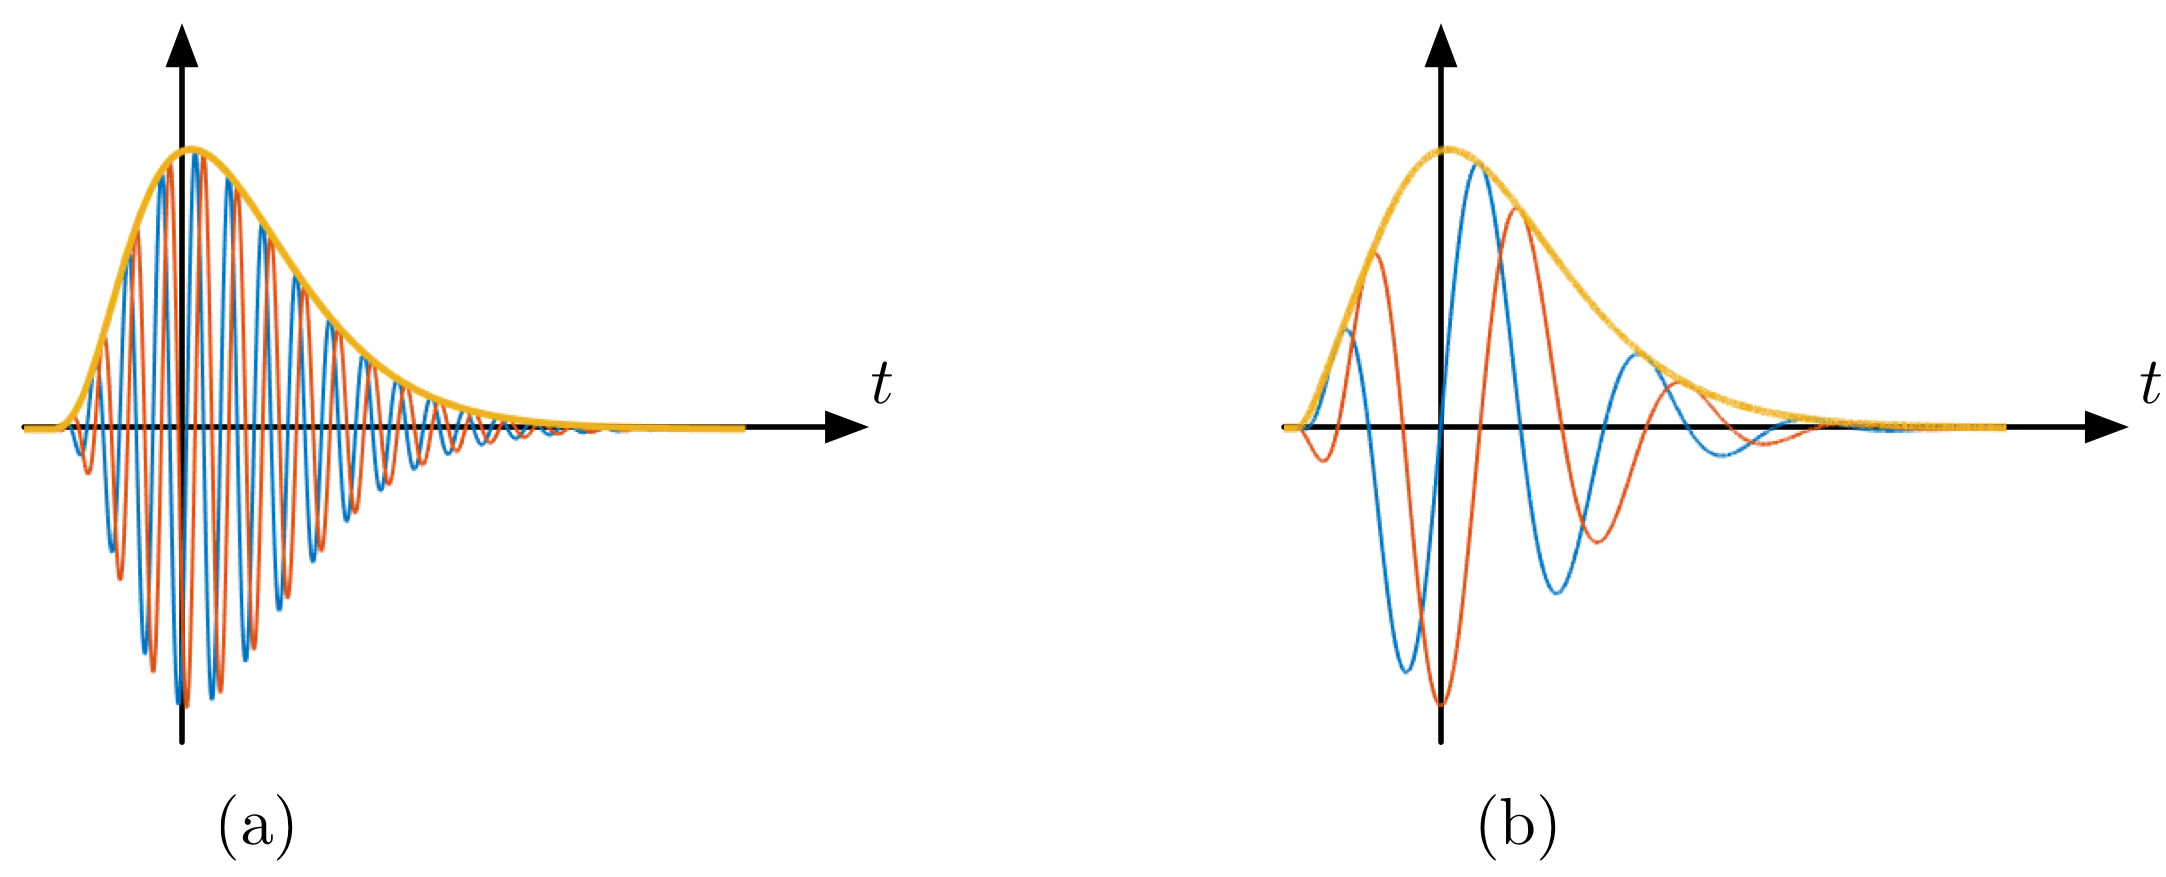
\includegraphics[width=\columnwidth]{gammatones}
%\caption{
%\label{fig:gammatones}
%Gammatone wavelets $\psi(t)$ in the time domain with quality factors (a) $Q = 4$ and (b) $Q = 1$. Blue and red oscillations represent the real and imaginary parts. The orange envelope represents the complex modulus.}
%\end{center}
%\end{figure}

\gl{TODO: Wavelets $\boldsymbol{\psi_{\gamma_1}}(t)$ and $\boldsymbol{\psi_{\gamma_2}}(t)$ are designed as fourth-order Gammatone
wavelets with one vanishing moment \cite{Venkitaraman2014}, and are shown in Figure \ref{fig:gammatones}.
In the context of auditory scene analysis, the asymmetric envelope of Gammatone wavelets is more biologically plausible than the symmetric, Gaussian-like envelope of the more widely used Morlet wavelets.
Indeed, it allows to reproduce two important psychoacoustic effects in the mammalian cochlea: the asymmetry of temporal masking and the asymmetry of spectral masking  \cite{Fastl2007}.
Moreover, it should be noted that Gammatone wavelets follow the typical amplitude profile of natural sounds, beginning with a relatively sharp attack and ending with a slower decay.
As such, they can be discovered automatically by unsupervised encoding of natural sounds \cite{Smith2006}.
This suggests that, despite being hand-crafted and not learned, Gammatone wavelets provide a sparse time-frequency representation of acoustic scenes.}

\subsubsection{Logarithmic compression}
\label{sec:ch6_LogComp}

\gl{TODO: Many algorithms in pattern recognition, including nearest-neighbor classifiers and SVMs, tend to work best when all features follow a standard normal distribution across all training instances \cite{Hsu2003}.
Yet the distribution of the scattering coefficients is skewed towards larger values. We can reduce this skewness by applying a pointwise concave transformation, such as a logarithm, to all coefficients.
Figure \ref{fig:histograms} shows the distribution of an arbitrarily chosen scattering coefficient over the DCASE 2013 dataset, before and after logarithmic compression.}

%\begin{figure}
%\begin{center}
%\includegraphics[width=\columnwidth]{compression}
%\caption{
%\label{fig:histograms}
%Histogram of values taken by the first-order scattering coefficient $\mathbf{S}\boldsymbol{x}(\gamma)$, corresponding to a center acoustic frequency of $302\,\mathrm{Hz}$,
%(a) before and (b) after logarithmic compression.}
%\label{fig:compression}
%\end{center}
%\end{figure}


\gl{TODO: Taking the logarithm of a magnitude spectrum is ubiquitous in audio signal processing.
Indeed, it is corroborated by the Weber-Fechner law in psychoacoustics, which states that the sensation of loudness is roughly proportional to the logarithm of the acoustic pressure. 
We must also recall that the measured amplitude of sound sources often decays polynomially with the distance to the microphone -- a source of spurious variability in scene classification.
Logarithmic compression can linearize this dependency, facilitating the construction of a powerful invariant at the classifier stage.}

\gl{TODO: For the task of musical genre recognition, second-order scattering coefficients $\mathbf{S_2}\boldsymbol{x}(t,\gamma_1,\gamma_2)$ are sometimes normalized by the corresponding first-order scattering coefficients $\mathbf{S_1}\boldsymbol{x}(t,\gamma_1)$, since this decorrelates them from one another \cite{Anden2014}.
We note that taking the logarithm of such renormalized coefficients yields}

\begin{equation}
\log \dfrac{\mathbf{S_2}\boldsymbol{x}(t,\gamma_1,\gamma_2)}{\mathbf{S_1}\boldsymbol{x}(t,\gamma_1)} =
\log \mathbf{S_2}\boldsymbol{x}(t, \gamma_1, \gamma_2) -
\log \mathbf{S_1}\boldsymbol{x}(t, \gamma_1),
\end{equation}

\gl{TODO: \ie a linear combination of the logarithms of first- and second-order coefficients.
As such, a non-linear renormalization becomes a linear transformation, which can be learned by a linearly discriminative classifier.}

\section{Algorithmes et classifieurs}

\subsection{Modèle de Markov caché}
\label{sec:ch6_hmm}

\gl{TODO: \citep{Rabiner1989}}

\subsection{Machines à vecteurs de support}
\label{sec:ch6_svm}

\subsection{Factorisation de matrice non-négative}
\label{sec:ch6_nmf}

\subsection{Autres classifieurs}
\label{sec:ch6_autresAlgo}

\gl{TODO: random forest, GMM}

\section{Détection des événements sonores}
\label{sec:ch6_AED}

\subsection{Objectifs}
\label{sec:ch6_objAED}

\gl{TODO: AED}

\subsection{Métrique}
\label{sec:ch6_metriqueAED}

Les performances des algorithme en AED sont évaluées suivant différentes métriques. Deux d'entre elles sont particulièrement utilisées, et notamment dans les challenges DCASE 2013 (\cf~Section~\ref{sec:ch6_dcase2013AED}) et 2016 (\cf~Section~\ref{sec:ch6_dcase2016AED}). Nous les détaillons dans cette section.

La première métrique est la F-mesure \citep{Giannoulis2013database,giannoulis2013detection,Stowell15}, que l'on note $F$ dans ce document. Cette dernière ce calcule comme suit:

\begin{equation}
F=\dfrac{2\times P \times R}{P+R}
\end{equation}

Où $P$ et $R$ représentent respectivement la précision et le rappel. La precision rend compte du rapport entre le nombre d'événements correctement détectés $c$ et le nombre d'événements effectivement détectés par l'algorithme $e$, tandis que le rappel rend lui compte du rapport entre le nombre d'événements correctement détectés $c$ sur le nombre d'événements à détecter $r$ (le nombre d'événements présents dans la scène):

\begin{equation}
P=\dfrac{c}{e}  \quad \textrm{, } \quad R=\dfrac{c}{r} \quad \textrm{, } \quad  e=c+fp \quad \textrm{, } \quad  r=c+fn
\end{equation}

avec $fp$ le nombre de faux positifs, et $fn$ le nombre de faux négatifs.


La deuxième métrique est le taux d'erreur acoustique \citep{poliner2007discriminative,clear}, que l'on note $ER$ dans ce document. Ce dernier ce calcule comme suit:

\begin{equation}
ER=\dfrac{D+I+S}{N}
\end{equation}

avec $N$ le nombre d'événements à détecter \gl{TODO: vérifier}, $D$ le nombre d'événements manqués ($fn$), $I$ le nombre d'événements faussement détectés ($fp$), et $S$ le nombre d'événements substitués, que l'on définit comme $S=min\lbrace D,I\rbrace$.

$F$ et $ER$ peuvent être calculées de deux manières suivant que l'on tienne compte: 

\begin{itemize}
\item du nombre de trames correctement identifiées ($sb$: \emph{segment based});
\item du nombre d'événements correctement identifiées ($eb$: \emph{event based}).
\end{itemize}

Considéré le nombre d'événements plutôt que les trames permets entre autres d'obtenir une mesure de performance indépendante de la durée des événements. Dans ce cas, on considère usuellement qu'un événement est correctement identifié si son \emph{onset} a été correctement identifié, ou si à la fois son \emph{onset} et son \emph{offset} ont été correctement identifiés. La détection d'une frontière (\emph{onset} ou \emph{offset}), est toujours considérée avec un seuil de tolérance.

Ainsi nous notons $F_{sb}$ et $ER_{sb}$, les F-mesures et taux d'erreur acoustiques calculés en tenant compte des trames, et $F_{eb}$ et $ER_{eb}$ les F-mesures et taux d'erreur acoustiques calculés en tenant compte des événements.

La détection de l'offset d'un événement sonore étant est un tâche compliquée, que ce soit pour des algorithmes ou des humains, nous ne considérons dans ce document des mesures de $F_{sb}$ et $ER_{sb}$ calculés en fonction du nombre d'événements dont les \emph{onsets} ont été correctement identifiés.

Enfin, il est possible de calculer ces métriques en 

Ces métriques, si elles sont calculés sans faire de distinction entre les classes, sont susceptible de donner des poids distincts dans l'évaluation entre les classes bien représentées dans la scène, et celles présentant que peu d'événement. Afin de parer à ce biais, il est possible de calculer les métriques séparément pour chaque classe, avant de les moyenner. On note ainsi $Fcw$ et $ERcw$, les versions alternatives de $F$ et $ER$ normalisée par classe:

\begin{equation}
\label{eq:ch7_eq3}
Fcw=\dfrac{1}{C}\sum_{i=1}^C F^i \quad \textrm{, } \quad ERcw=\dfrac{1}{C}\sum_{i=1}^C ER^i
\end{equation}

avec $C$ le nombre de classes à détecter et $F^i$ et $ER^i$, la F-measure et le taux d'erreur acoustique obtenus par un système en ne considérant que la classe d'événements $i$. 

Au final, 8 métriques sont donc disponibles pour évaluer les algorithmes en AED:, nommément $F_{sb}$, $F_{eb}$,$Fcw_{sb}$, $Fcw_{eb}$, $ER_{sb}$, $ER_{eb}$, $ERcw_{sb}$ et $ERcw_{eb}$.

\subsection{Tâche 3 du challenge DCASE 2013}
\label{sec:ch6_dcase2013AED}

\citep{Giannoulis2013database, giannoulis2013detection, Stowell15}
\gl{TODO: DCASE 2013, fenêtre de tolérance de $\pm100$ms \citep{Giannoulis2013database,Stowell15} }

\subsection{Tâche 3 du challenge DCASE 2016}
\label{sec:ch6_dcase2016AED}

\section{Classification des scènes sonores environnementales}
\label{sec:ch6_ASC}

\subsection{Objectifs}
\label{sec:ch6_objASC}

\gl{TODO: ASC}

\subsection{Métrique}
\label{sec:ch6_metriqueASC}

\subsection{Tâche 1 du challenge DCASE 2013}
\label{sec:ch6_dcase2013ASC}

\subsection{Tâche 1 du challenge DCASE 2016}
\label{sec:ch6_dcase2016ASC}

\section{Recouvrement des similarités acoustiques}
\label{sec:ch6_ASSR}

\subsection{Objectifs}
\label{sec:ch6_objASSR}

\gl{TODO: ASSR}

\subsection{Métrique}
\label{sec:ch6_metriqueASSR}

The metric used is the precision at rank $k$ ($p@k$), which is computed by taking a query item and counting the number of items of the same class within the $k$ closest neighbors, and then averaging over all query items. 

\subsection{Méthodes et algorithmes}
\label{sec:ch6_algoASSR}




%*****************************************
%*****************************************
%*****************************************
%*****************************************
%*****************************************




